\documentclass[Rapport/Rapport_main.tex]{subfiles}

\begin{document}

\subsection{Cup Sensor}
Lyset for hvert CupLight skal bl.a. styres på baggrund af om der er placeret en kop og om en bold er ramt i en kop. Derudover skal RPi vide hvilke kopper der er placeret på en given playerside da den skal vide hvornår spillet er færdigt.
\subsubsection{Hardware Design}
For at detektere placering af kop, og at at bold rammer i en kop, er der udført en teknologiundersøgelse. I denne undersøgelse, overvejes forskellige egenskaber en kop med øl har, som kan måles. Det overvejes bl.a. at koppen har en masse, koppen påvirker lys, og koppen har en anden dielektricitetskonstant end luft. Der undersøges i detalje sensorer der måler de to sidste egenskaber, en kapacitiv sensor og en optisk sensor. Disse to sensorer sammenlignes og bl.a. fordi den optiske sensor viste bedste tegn til at detektere at en bold rammer i, på trods at et lavere signal-støjforhold, vælges denne metode.

For at lave en optiske sensor benyttes der en IR LED som lyser op i centrum af koppen og fire fotodioder som er sensitive over for det lys som LED'en udsender. Der blev i teknologiundersøgelsen kun brugt 2 fotodioder på hver side af LED'en, men det blev observeret at signalet fra sensoren varierede meget afhængig af hvor bolden er i koppen. Derfor blev der benyttet 4, som placeret i en ring rundt om LED'en. Det blev i teknologiundersøgelsen også bestemt at den optimale afstand mellm LED og en fotodiode er ca. 10mm (4 modulafstande). Kredsløbet kan ses på figur \ref{fig:CupSensorDesign}  
\begin{figure}[H]
    \centering
    \makebox[\textwidth][c]{%
        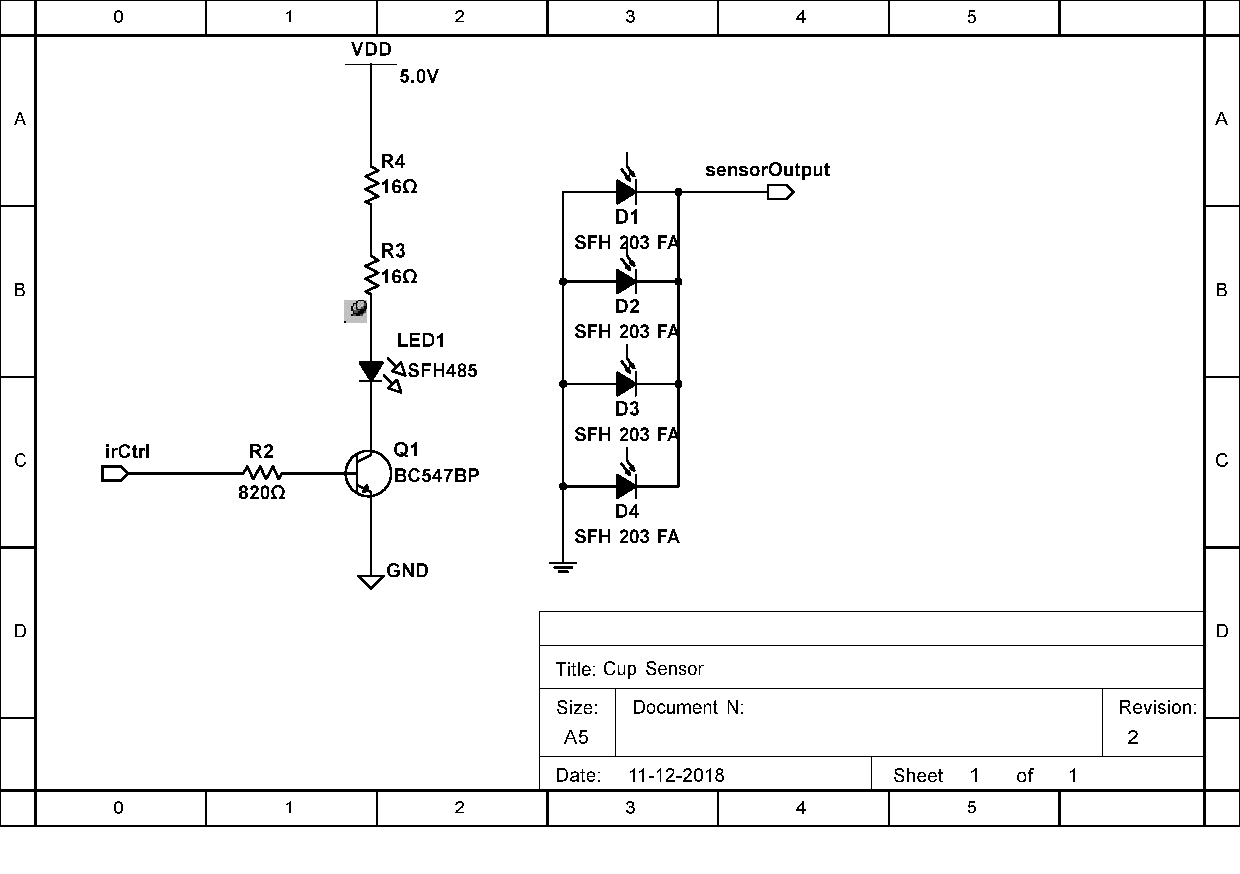
\includegraphics[width=1\columnwidth,trim={0.6in 1.8in 2.6in 0.25in},clip, page=1]{HardwareDesign/CupSensor/graphics/FinalDesign/CupSensor.pdf}
    }
    \caption{Design af Cup Sensor.}
    \label{fig:CupSensorDesign}
\end{figure}

Fotodioder virker på den måde at der i spæreretningen løber en strøm afhængig af lysintensiteten. Omgivelserne kan variere meget, og der kommer et DC offset, hvis systemet fx. bruges udendørs i sollys. Derfor er det valgt at blinke med LED'en, som styres vha. 'irCtrl', og nyttesignalet er derfor et AC signal. Til at sortere DC'en væk, bruges kredsløbet som ses på figur \ref{fig:CupSensorCupHolderControllerPart}, som fungerer som et højpas filter. Her forbindes 'sensorOutput' fra figur \ref{fig:CupSensorDesign} fra alle 6 Cup Sensor's til 'sensors' på figur \ref{fig:CupSensorCupHolderControllerPart}, som er en del af Cup Holder Controller 

\begin{figure}[H]
    \centering
    \makebox[\textwidth][c]{%
        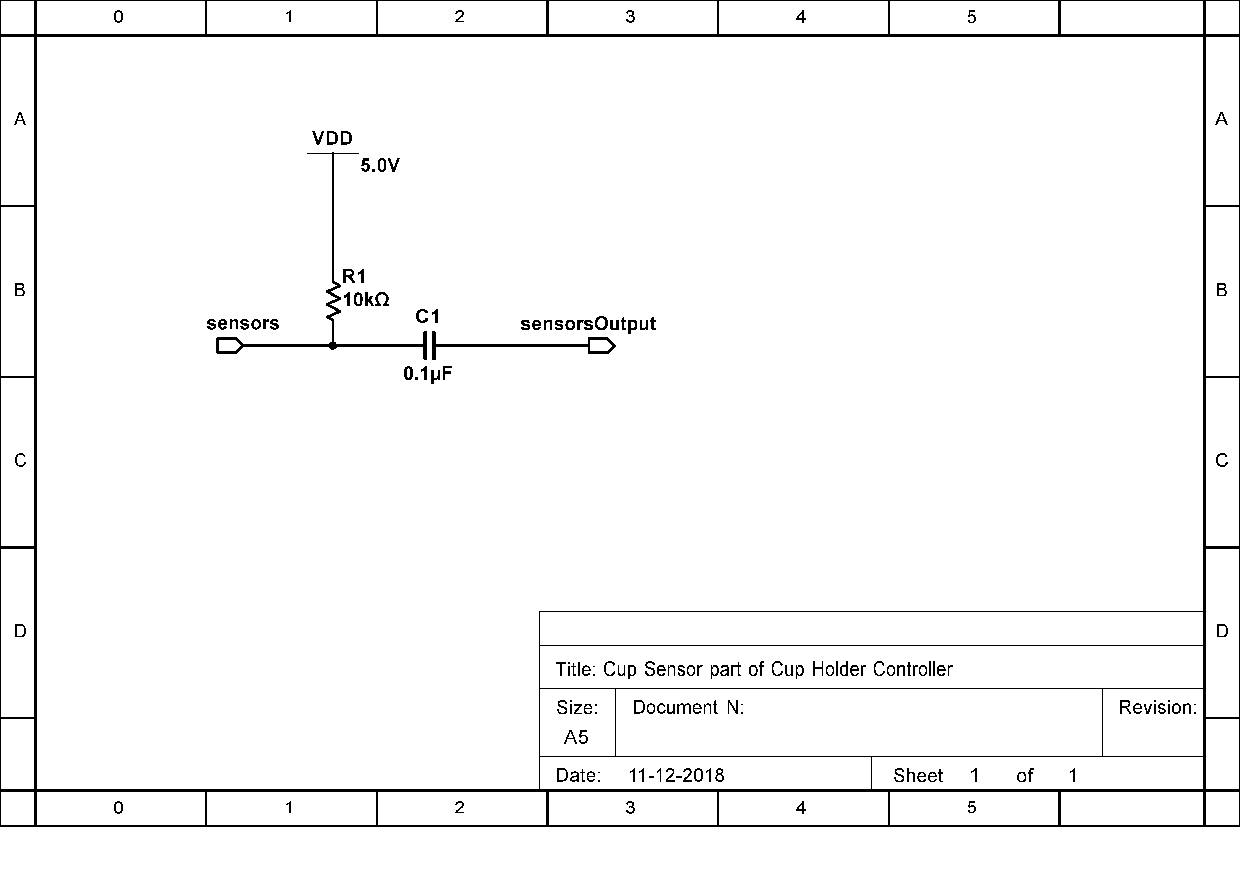
\includegraphics[width=0.7\columnwidth,trim={1.3in 3in 3.8in 0.5in},clip, page=1]{HardwareDesign/CupSensor/graphics/FinalDesign/CupSensorPart-CupHolderController.pdf}
    }
    \caption{Den del af Cup Holder Controller som sørger for at modtage signalet fra alle sensorer og filtrere DC fra.}
    \label{fig:CupSensorCupHolderControllerPart}
\end{figure}

Derudover benyttes der på PSoC'en en TIA til at konvertere strømsignalet til en spænding.Vha. mixerfunktionallitet indbygget i en Delta Sigma ADC laves der et båndpasfilter. På denne måde er DC niveauet fra ADC'en kun afhængig af det lys der sendes fra den infrarøde LED, da DC signaler og fx. 50Hz lys sorteres fra.

PSoC Komponenten kan ses på figur \ref{fig:CupSensorPSoCDesign}. Det ses at der bruges en demultiplexer, hvor hvert output ledControl0, ledControl1 ... styre LED'erne på hver Cup Sensor. På denne måde kan det vha. Control\_Red\_Led styres hvilken Cup Sensor's LED der skal blinke og dermed modtages der kun signalet fra denne sensor, selvom alle fotodioderne er forbundet til hinanden.  

\begin{figure}[H]
    \centering
    \makebox[\textwidth][c]{%
        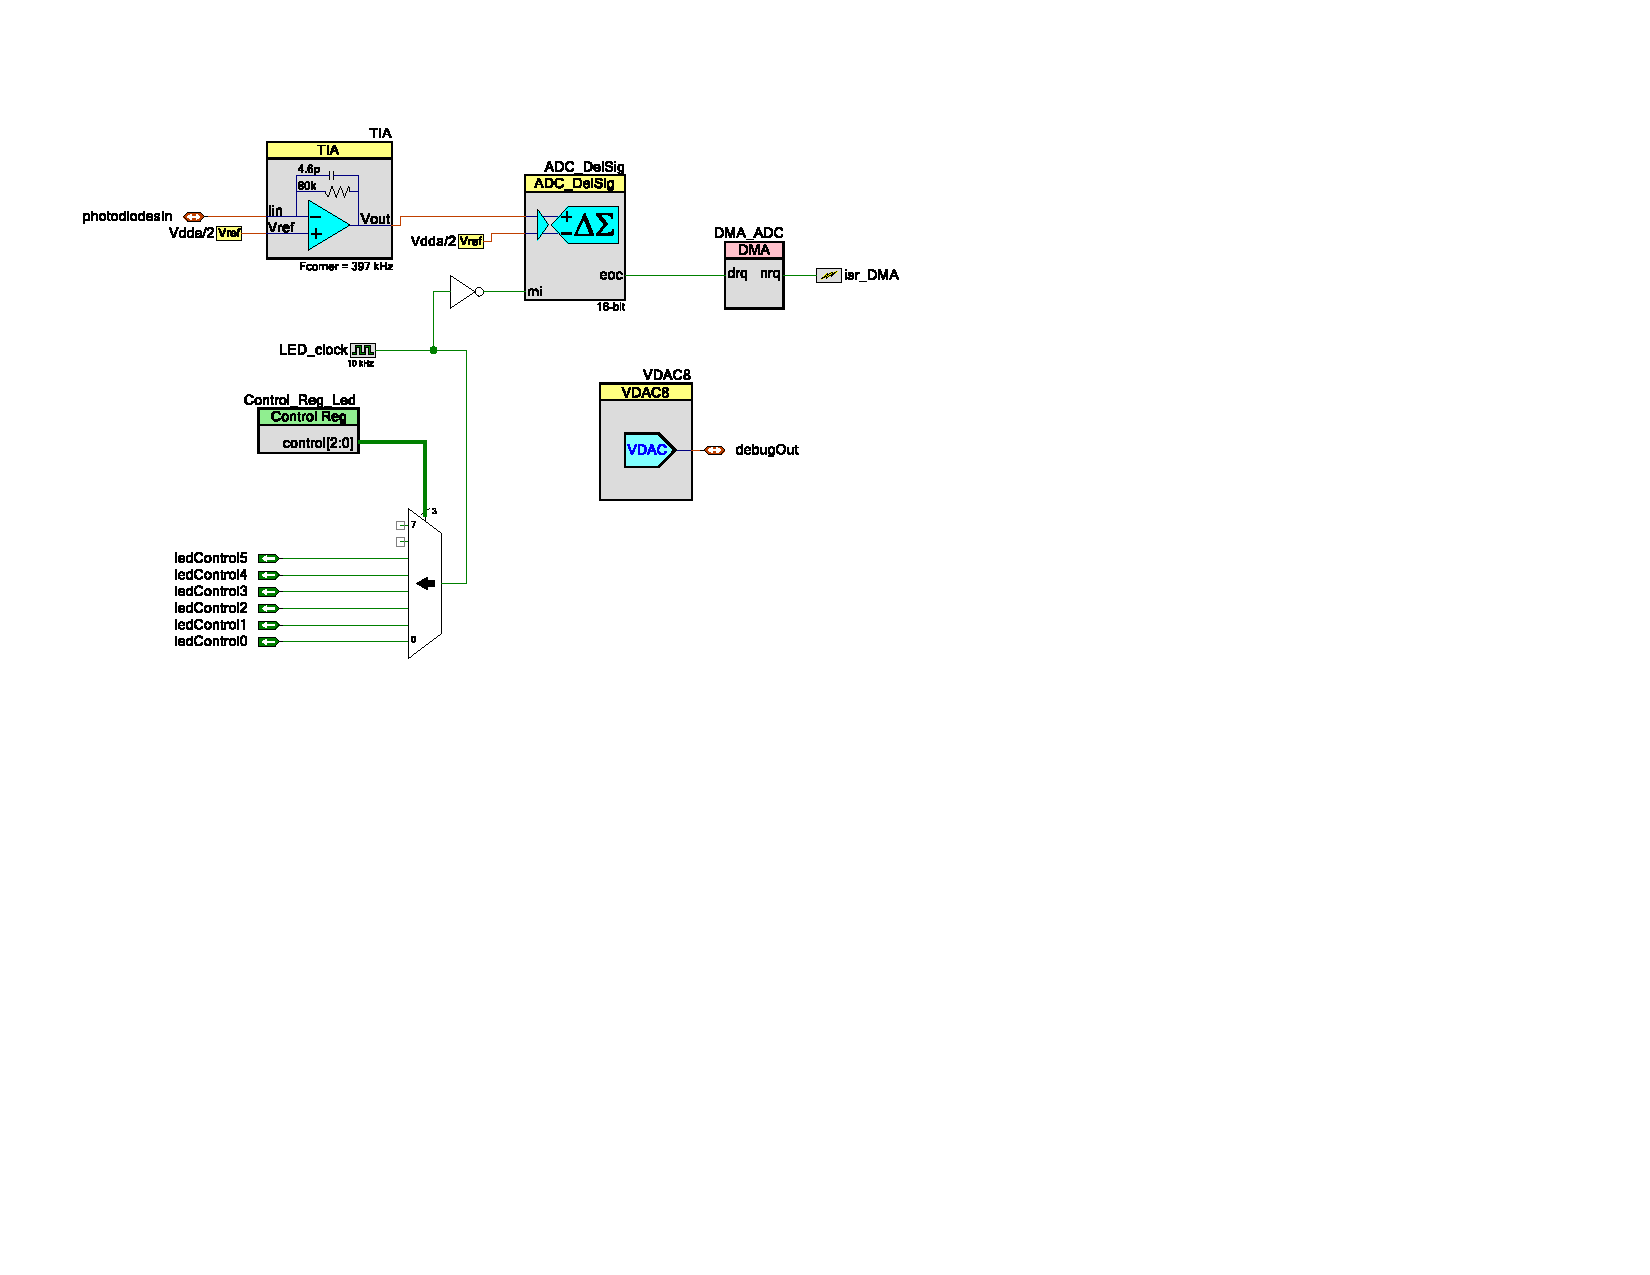
\includegraphics[width=1\columnwidth,trim={0.5in 4.1in 4.5in 0.8in},clip, page=1]{HardwareDesign/CupSensor/graphics/FinalDesign/PSoC-design.pdf}
    }
    \caption{PSoC design. 'photodiodesIn' forbindes til 'sensorsOutput' på figur \ref{fig:CupSensorCupHolderControllerPart}}
    \label{fig:CupSensorPSoCDesign}
\end{figure}

\subsubsection{Software Design}
Der er til software design af CupLight\_IF, udviklet et klassediagram. Diagrammet kan ses på figur \ref{fig:CupSensor-IF-classDiagram}. Det vil være uhensigtsmæssigt at lave alt i en klasse. Klassen CupSensor\_IF er den klasse som GameController interagere med. De resterende klasser er en del af en custom component i PSoC se afsnit \ref{sec:CupSensorImplementering}. CupSensor er hoved-klassen for CupSensor blokken. Den skal som alle andre PSoC komponenter startes vha. Start metoden. Derudover skal skal der være get metoder til Status og HitStatus. Derudover er to metoder med funktionspointere, som bruges til at indstille hvilke funktioner der skal kaldes når der skifter status. Til sidst er der en ISR som kaldes når der kommer en ny målling fra ADC'en. 
 
\begin{figure}[H]
    \centering
    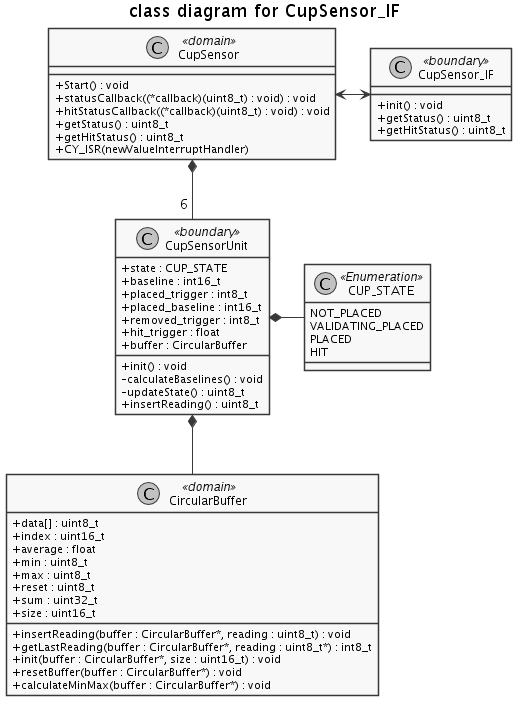
\includegraphics[width=0.8\textwidth]{Softwaredesign/CupSensor_IF/graphics/classDiagram.png}
    \caption{.}
    \label{fig:CupSensor-IF-classDiagram}
\end{figure}

Der er 6 objekter af klassen CupSensorUnit. Denne repræsentere hver Cup Sensor. Hver CupSensorUnit har en CUP\_STATE til at holde styr på tilstanden af den givne Cup Sensor. Derudover er der en CircularBuffer klasse som bruges til at lagre de seneste målinger for hver CupSensorUnit.

Der kan ses på sekvensdiagrammet på figur \ref{fig:CupSensor-IF-getting-reading} hvad der sker når der modtages en ny måling fra ADC'en. Den vigitge del i diagrammet er at når der modtages en målling fra en sensor, ændres der hvilken sensor der laves en måling på næste gang ved at styre Control\_Reg\_Led (se figur \ref{fig:CupSensorPSoCDesign}). Dette register styrer hvilken sensor der skal blinke. Derudover kaldes også insertReading metoden i den CupSensorUnit som læsningen stammer fra, bestemt af værdien af Control\_Reg\_Led. Denne metode returnerer om tilstanden ændres, hvis den gør kaldes de nødvendige metoder i GameController. 
\begin{figure}[H]
    \centering
    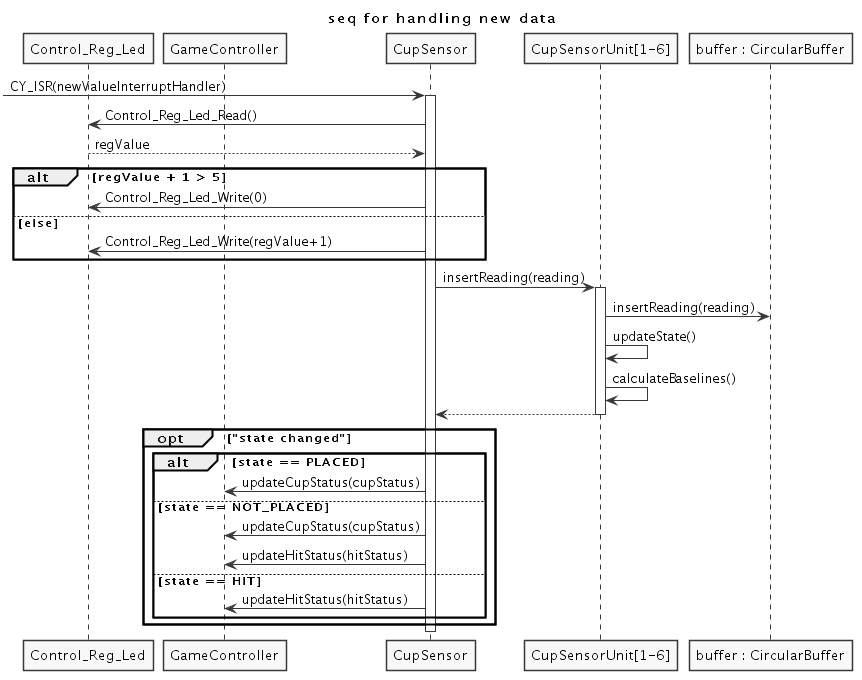
\includegraphics[width=1\textwidth]{Softwaredesign/CupSensor_IF/graphics/getting_reading.png}
    \caption{.}
    \label{fig:CupSensor-IF-getting-reading}
\end{figure}

Til at styre tilstanden for CupSensorUnit udvikles en tilstandsmaskine som ses på figur \ref{fig:CupSensor-IF-state}. Der er af åbenlyse grunde de tre tilstande NOT\_PLACE, PLACED og HIT. Men der er også en tilstand VALIDATING\_PLACED. Denne tilstand er til for at minimere risikoen for at der sker en falsk transition til tilstanden PLACED, da det kræver at signalet skal være højt i en længere tid, 20 samples eller ca. 300ms. Dette vil gøre systemet langsommere, men mere pålideligt. Som det ses på figur \ref{fig:CupSensor-IF-state}, benyttes der det der kaldes 'baseline', som er inspiration fra CapSense, som blev undersøgt i teknologiundersøgelsen. Der der benævnes 'reading', er den målte værdi minus den beregnede 'baseline'. Til at skifte mellem de forskellige tilstande benyttes der forskellige grænseværdier som reading skal være over/under. Til at skifte til tilstanden VALIDATING\_PLACED og tilbage til NOT\_PLACED, både fra VALIDATING\_PLACED, PLACED og HIT, benyttes der absolutte grænseværdier, placed\_trigger og removed\_trigger. Men til at skifte til HIT benyttes der en grænseværdi, hit\_trigger, der er relativ til værdien, placed\_baseline, når der er placeret en kop. Dette er til for at der fx. for en kop med meget øl, og derfor lille placed\_baseline, skal en mindre absolut ændring til for at detektere at en bold rammer i. Der vil komme en mindre ændring da bolden vil være længere væk fra sensoren.

\begin{figure}[H]
    \centering
    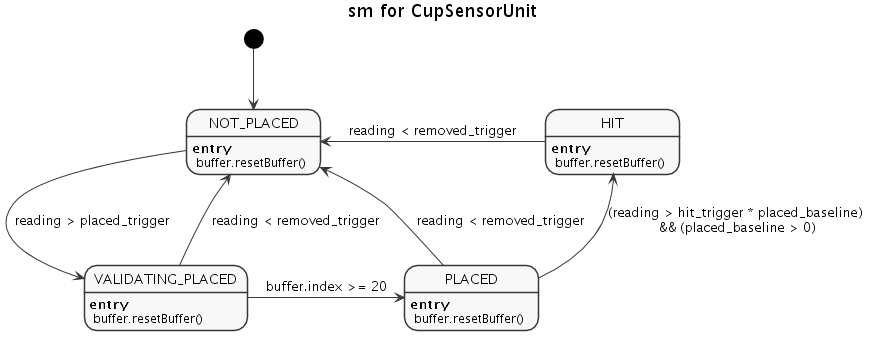
\includegraphics[width=1\textwidth]{Softwaredesign/CupSensor_IF/graphics/state.png}
    \caption{.}
    \label{fig:CupSensor-IF-state}
\end{figure}

Til at bestemme de forskellige grænseværdier der udført nogle målinger, hvor der placeres/fjernes en kop flere gange, og der tabes en bold flere gange. Dette udføres med forskellige mængder øl, den øvre og nedre grænse for mængden af øl beskrevet i kravene samt den nominelle værdi, 110ml. Det er forsøgt at bestemme grænseværdierne vha. konfidensniveau beregninger, i det der antages at målingerne er normalfordelte. Målingerne blev udført på et tidspunkt hvor der ikke var kendskab til denne type beregningerne, og det kan diskuteres om det er en realistisk antagelse at målingerne er normalfordelte. Derfor blev der hovedsageligt benyttet de maksimale og minimale målinger til at bestemme grænseværdierne.  

 

\subsubsection{Implementering}\label{sec:CupSensorImplementering}
Der er valgt at lav en custom PSoC komponent kaldet CupSensor. Dette er valgt da, der er mange delkomponenter som det ses på figur \ref{fig:CupSensorPSoCDesign}. Dette gør det meget uoverskueligt når det skal kombineres med resten af komponenterne på PSoC'en. Derudover vil det være relativt nemt at duplikere komponenten hvis der skulle ske ændringer som gør at der skal detekteres kopper i begge ender af bordet.

Da softwaren udvikles til PSoC vha. PSoC Creator er det (næsten) kun muligt at benytte C. Derfor implementeres klasserne i klassediagrammet, på figur \ref{fig:CupSensor-IF-classDiagram}, som moduler. Attributerne i de klasser der skal være flere af instanser af, CupSensorUnit og CircularBuffer, gemmes i structs. Den første parameter i metoderne i disse klasser, er en pointer til det struct der skal arbejdes på.


\paragraph{Printplade} Til at lave blokken Cup Holder, kombineres de to blokke Cup Light og Cup Sensor, som nu er blevet beskrevet. Der er designet printpladen som ses på figur \ref{fig:CupHolderPrintpladeDesign}. 

\begin{figure}[H]
\centering
\makebox[\textwidth][c]{%
\begin{subfigure}{.55\textwidth}
  \centering
        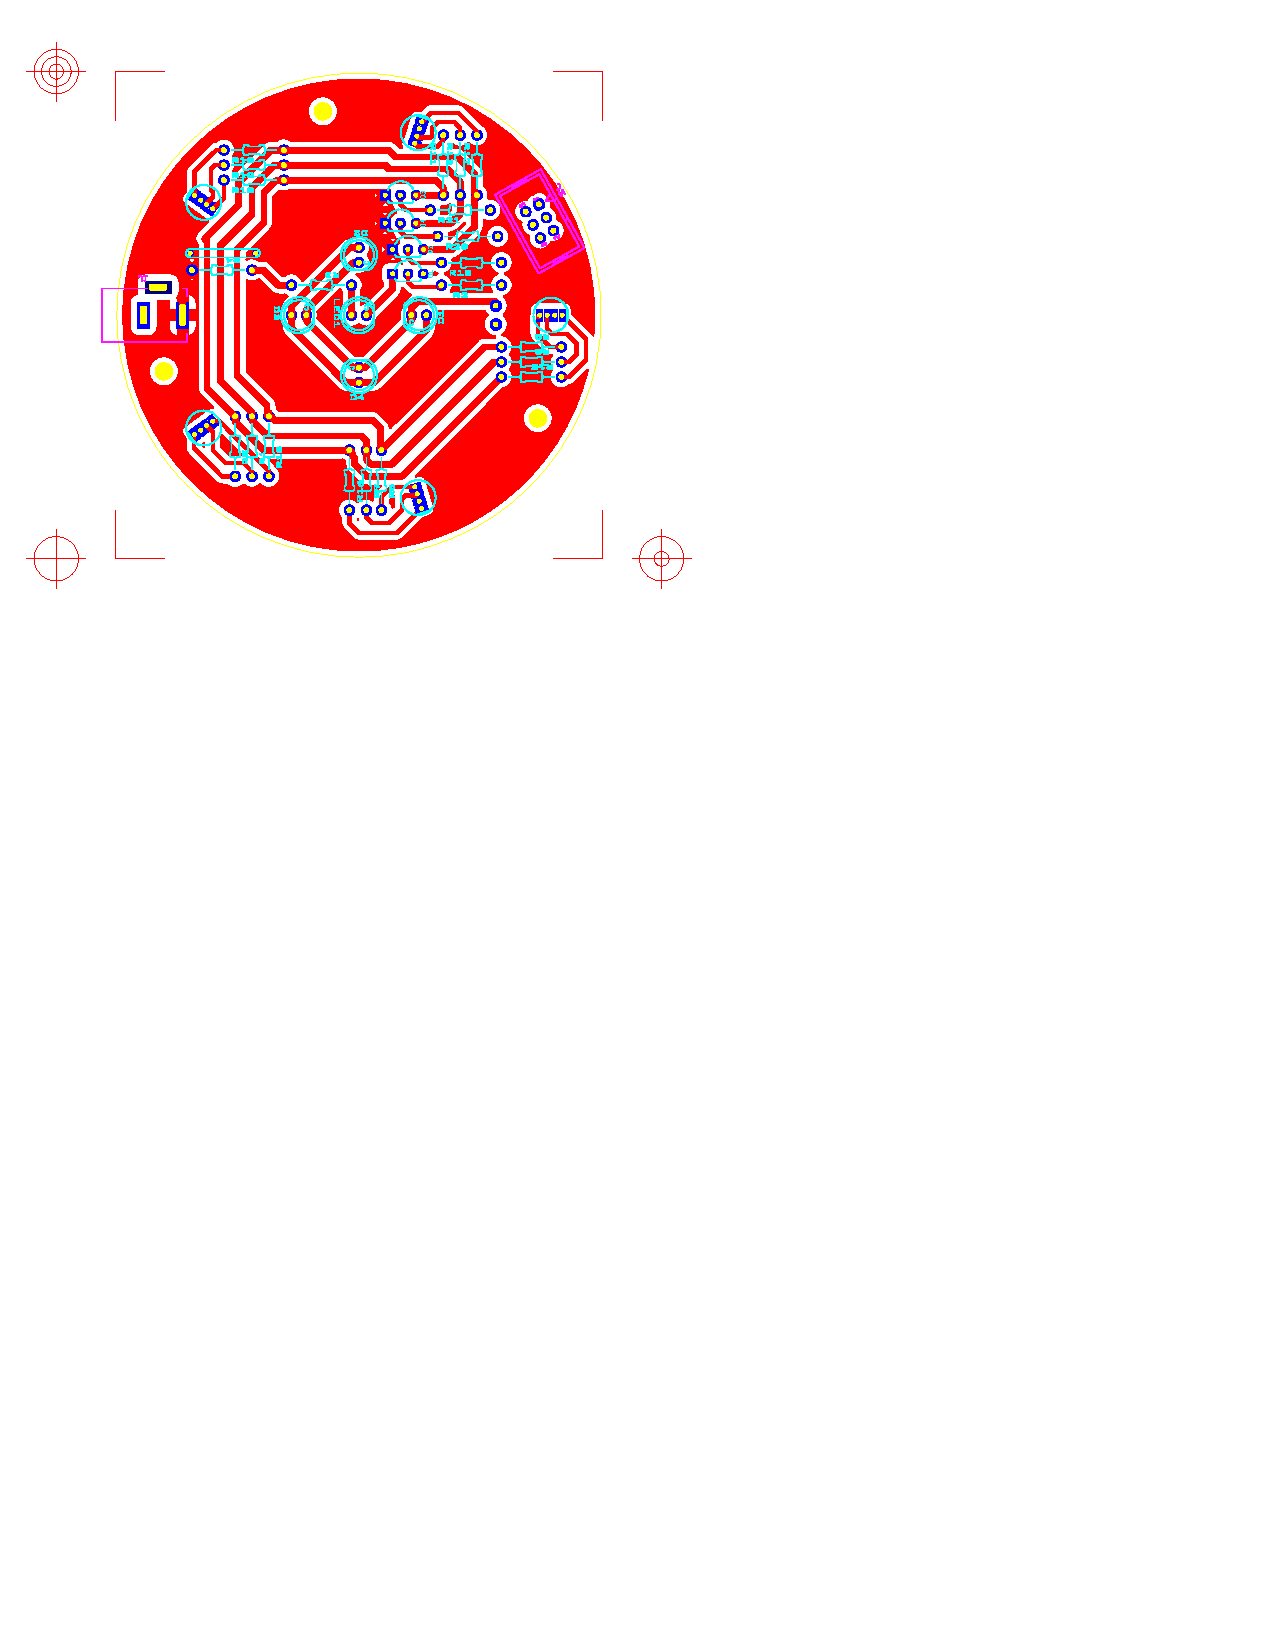
\includegraphics[width=1\linewidth,trim={0.6in 7.28in 4.5in 0.5in},clip, page=1]{HardwareDesign/CupHolder/graphics/bund.pdf}
\end{subfigure}%
\begin{subfigure}{.55\textwidth}
  \centering
    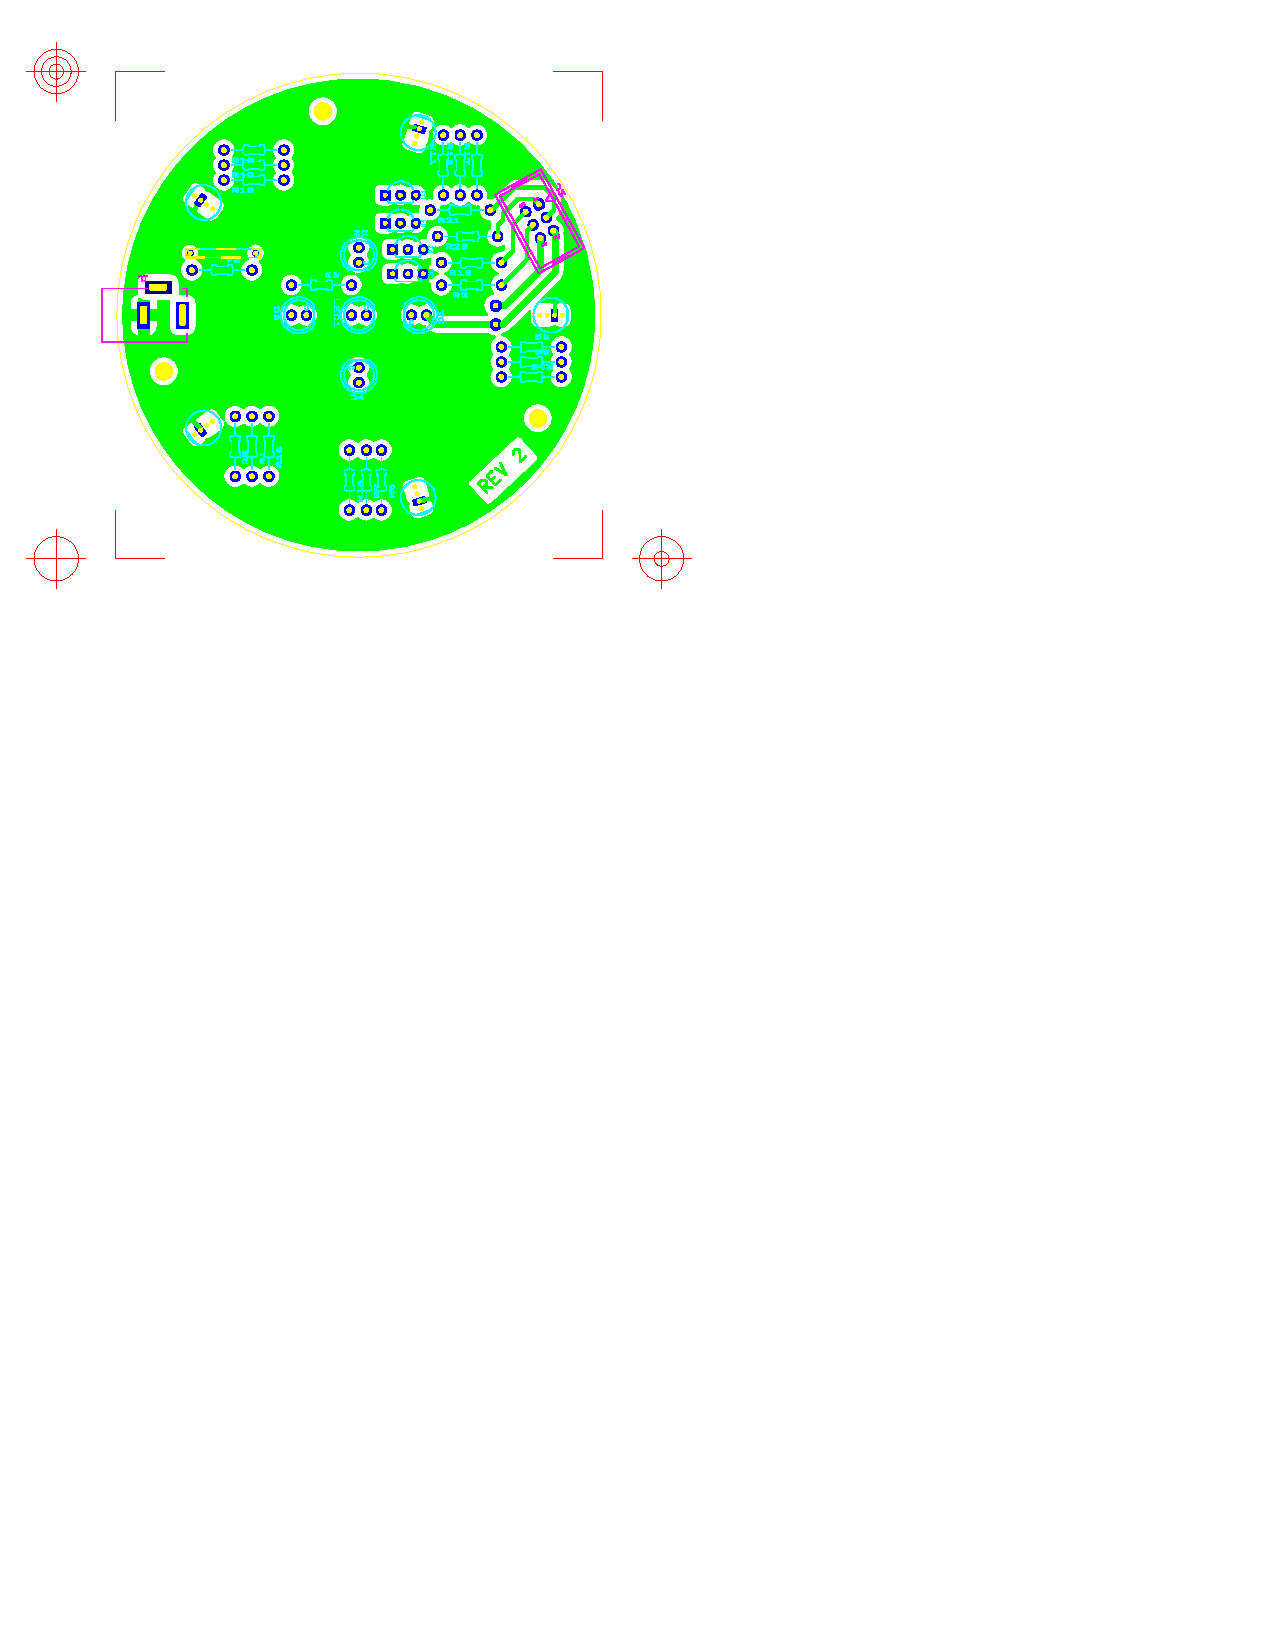
\includegraphics[width=1\linewidth,trim={0.6in 7.28in 4.5in 0.5in},clip, page=1]{HardwareDesign/CupHolder/graphics/top.pdf}
\end{subfigure}
}
\caption{Design af printplade. På venstre figur er det røde areal kobberet på undersiden af printpladen og på højre figur er det grønne areal kobberet på oversiden. Den cyane farve er silkscreen på toppen, som viser hvilke komponenter der er på oversiden. Den lilla farve er silkscreen på bunden og indikerer komponenter der sidder på bunden}
\label{fig:CupHolderPrintpladeDesign}
\end{figure}

Som en del af designet af printpladen er der fokus på minimering af støj, men også på de fysiske dimensioner. Der er i kravspecifikationen beskrevet hvordan de fem RGB LED'er skal være placeret i en cirkel med en diameter på ??. I designet af Cup Sensor er det også et krav at IR LED'en skal være i centrum og fotodioderne skal være 4 modulafstande fra IR LED'en. Derudover skal stikkene være i kanten af printpladen. Det er også valgt at printpladen skal være rund.

For at minimere støjpåvirkingen af PWM signalet til RGB LED'erne på sensoren er det forsøgt at flytte banerne til RGB LED'erne, de tre parallelle ydre baner, så langt væk fra banerne til sensorerne, de to parallelle indre baner. Dette ses et det vil være svært at have større afstand. Dette vil minimere den kapacitive kobling. Der kan stadig være noget induktiv støj. Denne støj mimimeres ved at returvejen af strømmene er så tæt på signalbanerne. Det vil for RGB LED'erne betyde at stel så tæt på de tre parallelle baner som muligt. Dette er udført da stort set hele den øvre kobber er et stelplan. For at have så kort en fælles stelvej som muligt er det også valgt at der er et seperat analog og digital stel. Det er dog i sidste ende det samme stel, men det får ført fælles stel på Cup Holder Controller.
Det er hermed forsøgt at minimere både den kapacitive og induktive kobling. For mere detaljeret forklaring refereres der til ?? i Hardwaredesign dokumentet.

Resultatet af printpladen kan ses på figur \ref{fig:CupHolderPrintplade}


\subsubsection{Modultest}
I modultesten testen sensoren ud fra de krav der er beskrevet i kravspecifikationen, samt de krav der er fra arkitekturen. Nogle af de mest relevante krav for sensoren er at systemet skal virke med $110\si{ml} \pm 20\si{ml}$ øl og sensoren skal virke med en forsyningsspænding på $5\si{V} \pm 0.2\si{V}$. Derfor testes de andre krav med alle kombinationer af $4.8\si{V}$, $5.0\si{V}$ og $5.2\si{V}$ og $90\si{ml}$, $110\si{ml}$ og $130\si{ml}$, altså i alt 9 kombinationer. De andre krav der testes er bl.a. antal detekteringer af placering og fjernelse af kop. Derudover testest det antal detekteringer af bolde der rammer i koppen.

Resultatet af modultesten viste at der detekteres placeringer og fjernelse 100 ud af 100 gange, med 0 falske detekteringer af at en bold rammer i, for alle af de 9 kombinationer. Deruover detekteres der i værste kombination, med $130\si{ml}$ øl og en forsyningsspænding på $5.2\si{V}$, 85 ud af 100 gange at en bold rammer i. I den næst værste kombination er det 93 og dernæst 96 ud af 100 gange. Det detekteres også hvor mange falske detekteringer der kommer når en bold kortvarigt rammer sensoren og hvor mange falske detekteringer der er i en time, både med og uden kop. Alle disse tilfælde var der 0 falske detekteringer.


\end{document}